\setcounter{chapter}{3}
\setcounter{section}{0}
\part{MÉTODOLOGÍA DE LA INVESTIGACIÓN} 

\section{Localización}

El proyecto se realizó en la Universidad Técnica Estatal de Quevedo (UTEQ), campus "La María", ubicada en el Cantón Mocache de la Provincia Los Ríos, en Ecuador. Previo a la obtención del titulo de Ingeniero en Sistemas. La ejecución del proyecto duró 4 meses, desde el mes de junio de 2022 hasta el mes de septiembre del 2022.

\begin{figure}[h!]
	\centering
	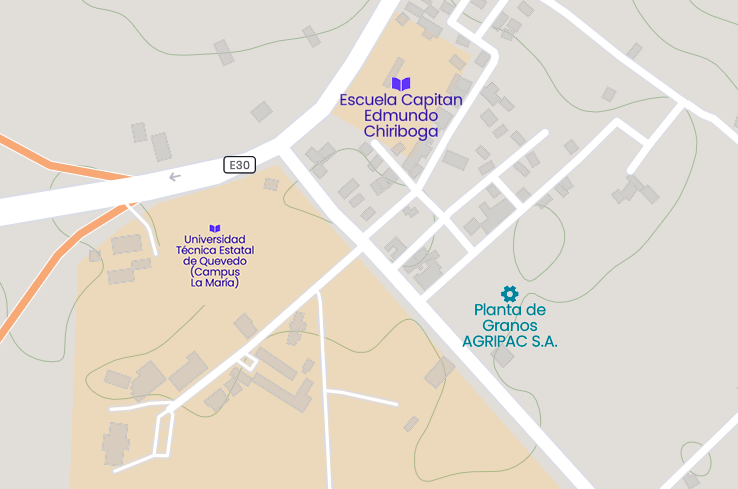
\includegraphics[width=12cm]{img/campuslamaria.png}
	\caption{Localización de la UTEQ campus "La María".}
	\label{fig:lamaria}
\end{figure}.

\section{Tipo de investigación}

La ejecución de este proyecto implico realizar una investigación de tipo exploratoria. Existen trabajos similares al presentado, pero no cumplen con conceptos semejantes a los que se ha planteado en este trabajo. Se utilizaron artículos científicos de revistas científicas indexadas y conferencias internacionales.

\section{Método de investigación}

\subsection{Método analítico}

\subsection{Método inductivo}

\section{Fuentes de recopilación de información}

\section{Diseño de la investigación}

Para el desarrollo del presente proyecto se tomarán en cuenta la ejecución de varias etapas, aplicando el Modelo de Prototipado para desarrollar un prototipo de la aplicación web que utilice el producto final de esta investigación. A continuación, se describe el enfoque metodológico correspondiente a cada una de las fases. 

\subsection{Búsqueda de aplicativos relacionados}

En esta fase se analizaron varias aplicaciones web que cuentan con la funcionalidad de generar diagramas de clases mediante la escritura de texto. Entre las aplicaciones analizadas se encuentran:

\begin{itemize}
	\item \textbf{yuml: }Es una aplicacion web que permite crear diagramas UML mediante la escritura por comandos en texto plano. Se puede destacar que esta herramienta no permite decidir la ubicación o lugar de un elemento grafico ya que busca la mejor distribución según el diagrama generado (https://yuml.me/)
	
	\item \textbf{mermaid: }Es una herramienta de gráficos y diagramas basada en JavaScript que utiliza definiciones de texto inspiradas en Markdown y un renderizador para crear y modificar diagramas complejos. El propósito principal de Mermaid es ayudar a que la documentación se ponga al día con el desarrollo. También se destaca que la aplicación no permite modificar en tiempo real los diagramas generados (https://mermaid.live/).
	
	\item \textbf{ditaa: }Es una pequeña utilidad de línea de comandos escrita en Java, que puede convertir diagramas dibujados con arte ascii ('dibujos' que contienen caracteres que se asemejan a líneas como | / - ), en gráficos de mapa de bits adecuados. También se destaca que la aplicación no permite modificar en tiempo real los diagramas generados (http://ditaa.sourceforge.net/). 
\end{itemize}

\subsection{Modelamiento}

En esta etapa se pretende modelar la funcionalidad que tendrán todos los métodos y funciones necesarias para identificar cada símbolo y poder interpretar todo el texto para generar la estructura del diagrama de clases.
Todo el archivo JavaScript estará conformado por estructuras de datos apuntando a la programación orientada a objetos.

\subsection{Desarrollo del código}

La tercera etapa se dedicará al desarrollo de la librería utilizando el lenguaje de programación JavaScript. Todo el código será escrito en un solo archivo con extensión de tipo .js teniendo como ventaja poder ser vinculado dentro de cualquier archivo HTML que dese utilizar los métodos necesarios para obtener la estructura de todo el diagrama de clases en formato JSON.

La estructura podrá ser utilizada por cualquier herramienta de dibujo externa que permita visualizar el diagrama de clases de la forma tradicional con todos sus componentes. A continuación, se enlista los componentes que podrán ser generados por la librería:

\begin{itemize}
	\item Entidades
	\item Interfaces
	\item Enumeradores
	\item Atributos
	\item Métodos
	\item Constructores de clases
	\item Relaciones
\end{itemize}

\subsection{Pruebas unitarias}
En esta fase se pretende realizar todas las pruebas posibles a las funciones que se realizaron en la fase anterior, ingresando algunos textos utilizando los símbolos esperando los valores que devuelva la librería. Algunos de los textos que serán ingresados son los siguientes:

\begin{itemize}
	\item \begin{verbatim}
		Create an user *(user %.username=String, .password=String,
		.status=Status, .user type=UserType, .person=Tutor%) object
	\end{verbatim}
	
	\item \begin{verbatim}
		*(TutorDAO &id=Int [/Save/=Tutor{.tutor=Tutor}])s the tutor 
		data in the database. *¡(TutorDAO)<<*(tutor)¡
	\end{verbatim}
	
	\item \begin{verbatim}
		*(UserDAO &-id=Int [/Save/=User{.user=User}])s the user data 
		in the database. *¡(UserDAO)<<*(User)¡
	\end{verbatim}
	
	\item \begin{verbatim}
		This use case ends when the system displays the *(@Login) 
		login Interface. *¡(Login)<<*(UserDAO)¡
	\end{verbatim}
	
\end{itemize}

\subsection{Evaluación con sistemas de información reales}

Se utilizaran estudios de caso con sistemas de información reales para crear las descripciones de los casos de uso extendidos de forma natural. Luego se implementaron los símbolos como se crea conveniente, dependiendo de los requisitos ingresados en el texto. Finalmente se utilizara la librería para observar como devuelve el texto nuevamente en forma natural adicional la estructura del diagrama de clases.

\subsection{Modelo de prototipado}
El Modelo de Prototipado se aplica cuando la información detallada relacionada a requerimientos de entrada y salida del sistema no está disponible. En este modelo se asume que tal vez no todos los requerimientos son conocidos en el inicio del desarrollo del sistema. Se usa generalmente cuando un sistema no existe, o en caso de un largo y complejo sistema, cuando no hay procesos manuales para determinar los requerimientos. Los pasos que se ejecutan en el modelo de prototipado son: 

\begin{enumerate}
	\item \textbf{Obtención y análisis de requisitos:} es el punto de partida del modelo. El usuario es entrevistado para conocer los requisitos del sistema.
	
	\item \textbf{Diseño rápido}: teniendo claro todos los requisitos, se procede a crear un diseño rápido y preliminar incluyendo solo los aspectos más importantes 
	
	\item\textbf{ Construir el prototipo:} se trabaja con la información tomada por el diseño rápido y crear el prototipo de la aplicación.
	
	\item \textbf{Evaluación de usuarios}: el sistema es presentado a varios usuarios para evaluar y verificar sus puntos fuertes y débiles Se reciben comentarios y sugerencias que serán analizadas por los desarrolladores.
	
	\item \textbf{Reajuste del prototipo:} el prototipo actual debe reajustarse según los nuevos requerimientos, es decir que, se debe crear un nuevo prototipo con la información adicional proporcionada por los usuarios evaluados. Este nuevo prototipo será reevaluado justo como el anterior. Este proceso se repite hasta que se cumplan todos los requerimientos especificados por el usuario. Cuando el usuario esté satisfecho con el resultado, se desarrollará un sistema final basado en el prototipo final. 
	
	\item \textbf{Implementación y mantenimiento:} Una vez que se tenga listo el sistema, ya estará listo para ser desplegado a producción. El sistema se somete a un mantenimiento de rutina para minimizar el tiempo de inactividad y evitar fallas a gran escala.
	
\end{enumerate}